\pagenumbering{arabic}
%\setcounter{secnumdepth}{0}
\chapter{Svolgimento esercizi assegnati}
	\section{Esercizio 2.13}
		Formalizzare e dimostrare la validit\`a dell'induzione strutturale
		\emph{mutua} che consente la dimostrazione simultanea di diverse propriet\`a
		per diverse categorie sintattiche.
		
		\sectionline
		
		A volte si ha la necessit\`a di dimostrare congiuntamente un gruppo di
		enunciati $S1(n),S2(n),\ldots,Sk(n)$ per induzione su n. Un gruppo di
		enunciati potrebbe essere dimostrato, dimostrando la congiunzione ($AND$
		logico) di tutti gli enunciati ($S1(n)\land S2(n)\land \ldots \land Sk(n)$).
		Tuttavia di solito conviene tenere separati gli enunciati e dimostrare per
		ciascuno la rispettiva base e il passo induttivo. Questo tipo di dimostrazione
		\`e detto \emph{induzione mutua}.
		
		Consideriamo ad esempio un interruttore on/off, rappresentato con il seguente
		automa:
		
		\begin{figure}[h]
			\centering
			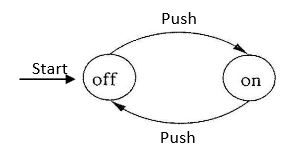
\includegraphics[scale=1]{img/Interruttore}
			\caption{Un semplice interruttore}
		\end{figure}
		
		Ad ogni pressione del pulsante lo stato cambia tra ON e OFF. Proviamo a
		dimostrare i seguenti due enunciati:
		
		$S1(n):$ \emph{l'automa si trova nello stato OFF dopo n pressioni}
		$\Leftrightarrow$ \emph{n \`e pari.}
		
		$S2(n):$ \emph{l'automa si trova nello stato ON dopo n pressioni}
		$\Leftrightarrow$ \emph{n \`e dispari.}
		
		Sapendo che un numero $n$ non pu\`{o} essere allo stesso tempo pari e dispari, si
		potrebbe supporre che $S1 \Rightarrow S2$, e viceversa. Questo per\`{o} non \`{e}
		sempre vero in quanto, in generale, un automa potrebbe trovarsi
		contemporaneamente in pi\`{u} stati. Non \`{e} questo il caso dell'automa preso come
		esempio che si trova sempre esattamente in un solo stato, ma questo deve
		essere dimostrato come parte dell'induzione mutua.
		
		Proviamo a dimostrare le precedenti propriet\`a:
		
		\textbf{BASE:} Per il caso base scegliamo $n=0$. Dato che ci sono due
		enunciati, ognuno dei quali deve essere dimostrato in entrambe le
		direzioni ($S1$ e $S2$ sono enunciati `se e solo se`), in effetti ci sono
		quattro casi per la base e altrettanti per l'induzione:
		\begin{enumerate}
		  \item $[S1(0), \Rightarrow]$ Dato che $0$ \`e pari, dobbiamo dimostrare che dopo $0$
		  pressioni l'automa si trova nello stato OFF. Lo stato iniziale dell'automa \`e proprio
		  OFF e quindi l'automa si trova effettivamente nello stato OFF dopo $0$
		  pressioni.
		  \item $[S1(0), \Leftarrow]$ L'automa si trova nello stato OFF dopo $0$
		  pressioni, quindi dobbiamo dimostrare che $0$ \`e pari. $0$ \`e pari per
		  definizione quindi non resta altro da dimostrare.
		  \item $[S2(0), \Rightarrow]$ L'ipotesi afferma che $0$ \`e un numero dispari
		  $\Rightarrow$ l'implicazione \`e vera.
		  \item $[S2(0), \Leftarrow]$ L'ipotesi afferma che l'automa si trovi
		  nello stato ON dopo $0$ pressioni. Questo \`e impossibile in quanto all'automa
		  serve almeno una pressione del tasto per arrivare nello stato ON
		  $\Rightarrow$ l'implicazione \`e vera.
		\end{enumerate}
		
		\textbf{PASSO INDUTTIVO:} Supponiamo che $S1(n)$ e $S2(n)$ siano vere, e
		proviamo a dimostrare $S1(n+1)$ e $S2(n+1)$. Anche questa dimostrazione si divide in 4
		parti:
		
		\begin{enumerate}
		  \item $[S1(n+1), \Rightarrow]$ Per ipotesi, $n+1$ \`e pari. Di conseguenza $n$ \`e
		  dispari.
		  $S2(n)$ dice che dopo $n$ pressioni l'automa si trova nello stato ON. L'arco
		  da ON a OFF etichettato `Push` dice che la n+1-esima pressione far\`a
		  passare l'automa nello stato OFF.
		  \item $[S1(n+1), \Leftarrow]$ L'ipotesi \`e che l'automa si trovi nello
		  stato OFF dopo $n+1$ pressioni. Esaminando l'automa vediamo che l'unico modo
		  di pervenire allo stato OFF \`e di trovarsi nello stato ON e di ricevere in
		  input il comando `Push`. Perci\`{o}, se l'automa si trova nello stato OFF dopo
		  $n+1$ pressioni, deve essersi trovato nello stato ON dopo $n$ pressioni.
		  Quindi da $[S2(n), \Leftarrow]$ concludiamo che $n$ \`{e} dispari. Dunque
		  $n+1$ \`e pari.
		  \item $[S2(n+1), \Rightarrow]$ L'ipotesi afferma che $n+1$ \`e dispari. Di conseguenza
		  $n$ \`e pari. $[S1(n), \Rightarrow]$ dice che dopo $n$ pressioni l'automa si trova
		  nello stato OFF. L'arco da OFF a ON con etichetta `Push` dice che la
		  $n+1$-esima pressione far\`a passare l'automa nello stato ON.
		  \item $[S2(n+1), \Leftarrow]$ L'ipotesi \`e che l'automa si trovi nello
		  stato ON dopo $n+1$ pressioni. Esaminando l'automa vediamo che l'unico modo
		  di pervenire allo stato ON \`e di trovarsi nello stato OFF e di ricevere in
		  input il comando `Push`. Perci\`{o}, se l'automa si trova nello stato ON dopo
		  $n+1$ pressioni, deve essersi trovato nello stato OFF dopo $n$ pressioni.
		  Quindi da $[S1(n), \Leftarrow]$ concludiamo che $n$ \`{e} dispari. Dunque
		  $n+1$ \`{e} pari.
		\end{enumerate}
		
		Da questo esempio possiamo ricavare il modello di tutte le induzioni mutue:
		
		\begin{itemize}
		  \item Ogni enunciato deve essere dimostrato separatamente nella base e nel
		  passo induttivo.
		  \item Se si tratta di enunciati `se e solo se`, allora entrambe le direzioni
		  di ogni enunciato devono essere dimostrate, sia nella base che nel passo
		  induttivo.
		\end{itemize}
		
		\newpage
		
	\section{Esercizio 3.13}
		Fornire l'espressione, derivante dalla sintassi concreta
		dell'esercizio $11$, che ha il seguente albero di derivazione:
		
		\begin{figure}[h]
			\centering
			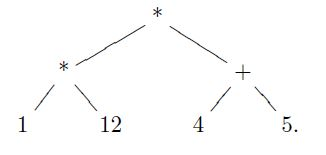
\includegraphics[scale=0.5]{img/3-13}
			\caption{Albero di derivazione}
		\end{figure}
		
		\sectionline
		
		L'espressione derivante \`e: $(1*12)*(4+5)$
		
		\newpage
	
	\newpage \section{Esercizio 4.6}
		Dimostrare che la semantica denotazionale delle espressioni regolari
		soddisfa le seguenti semplici propriet\`a:
		\subsection{punto (a)}
			$$E+(F+G) \simeq (E+F)+G$$
		\subsection{punto (e)}
			$$E(FG) \simeq (EF)G$$
		\subsection{punto (f)}
			$$E(F+G) \simeq EF+EG$$
			
		\sectionline
		
		La semantica denotazionale delle espressioni regolari \`{e} cos\`{\i} definita:
		\begin{itemize}
		  \item $\mathcal{L} \llbracket 0 \rrbracket = \emptyset$
		  \item $\mathcal{L} \llbracket 1 \rrbracket = \{\epsilon\}$
		  \item $\mathcal{L} \llbracket a \rrbracket = \{a\}$ (per $a \in A$)
		  \item $\mathcal{L} \llbracket E + F \rrbracket = \mathcal{L} \llbracket E
		  	\rrbracket \cup \mathcal{L} \llbracket F
		  	\rrbracket$
		  \item $\mathcal{L} \llbracket E ; F \rrbracket = \mathcal{L} \llbracket E
		  	\rrbracket \cdot \mathcal{L} \llbracket F
		  	\rrbracket$ 
		  \item $\mathcal{L} \llbracket E^* \rrbracket = (\mathcal{L} \llbracket E
		  	\rrbracket)^*$ 
		\end{itemize}
		
		Da queste equivalenze possiamo ricavare:
		\begin{itemize}
		  \item punto (a):$$ E+(F+G) \simeq (E+F)+G $$  		  
		  	\begin{align*}
		  		\mathcal{L} \llbracket E+(F+G) \rrbracket &= \mathcal{L}
		  		\llbracket E \rrbracket \cup \mathcal{L}
		  		\llbracket F + G \rrbracket \\ &= \mathcal{L}
		  		\llbracket E \rrbracket \cup \mathcal{L}
		  		\llbracket F \rrbracket \cup \mathcal{L}
		  		\llbracket G \rrbracket \\ &= \mathcal{L}
		  		\llbracket E + F \rrbracket \cup \mathcal{L}
		  		\llbracket G \rrbracket \\ &= \mathcal{L} \llbracket (E + F) + G
		  		\rrbracket
		  	\end{align*}
		  \item punto (e): $$E(FG) \simeq (EF)G$$
		  	\begin{align*}
		  		\mathcal{L} \llbracket E(FG) \rrbracket &= \mathcal{L} \llbracket E
		  		\rrbracket \cdot \mathcal{L} \llbracket FG \rrbracket \\ &= \mathcal{L} \llbracket E \rrbracket \cdot
		  		\mathcal{L} \llbracket F \rrbracket \cdot \mathcal{L} \llbracket G
		  		\rrbracket \\ &= \mathcal{L} \llbracket EF \rrbracket \cdot \mathcal{L}
		  		\llbracket G \rrbracket \\ &= \mathcal{L} \llbracket (EF)G \rrbracket
		  	\end{align*}
		  \item punto (f): $$E(F+G) \simeq EF + EG$$
		  	\begin{align*}
		  		\mathcal{L} \llbracket E(F+G) \rrbracket &= \mathcal{L} \llbracket E
		  		\rrbracket \cdot \mathcal{L} \llbracket F+G \rrbracket \\ &= \mathcal{L} \llbracket E
		  		\rrbracket \cdot (\mathcal{L} \llbracket F \rrbracket \cup \mathcal{L}
		  		\llbracket G \rrbracket) \\ &= (\mathcal{L} \llbracket E \rrbracket \cdot
		  		\mathcal{L} \llbracket F \rrbracket) \cup (\mathcal{L} \llbracket E
		  		\rrbracket \cdot \mathcal{L} \llbracket G \rrbracket) \\ &= \mathcal{L}
		  		\llbracket EF + EG
		  		\rrbracket
		  	\end{align*}
		\end{itemize}
		
		\newpage
			
	\section{Esercizio 5.7}
	
		Siano:
		\begin{equation*}
			\svar = \lambda xyz.xz(yz)
		\end{equation*}
		\begin{equation*}
			\kvar = \lambda xy.x
		\end{equation*}
		\begin{equation*}
			\ivar = \lambda x.x
		\end{equation*}
		Trovare la forma normale dei due termini:
		\begin{equation*}
			(\lambda y.yyy)(\kvar\ivar(\ssvar))\text{ e }\sssssssvar
		\end{equation*}
		
		\sectionline
		
		\begin{align*}
			(\lambda y.yyy)(\kvar\ivar(\ssvar)) & =
			(\kvar\ivar(\ssvar))(\kvar\ivar(\ssvar))(\kvar\ivar(\ssvar))\\
			& = ((\lambda y.\ivar)(\ssvar))((\lambda y.\ivar)(\ssvar))((\lambda
			y.\ivar)(\ssvar))\\
			& = \ivar\ivar\ivar\\
			& = \ivar\ivar\\
			& = \ivar\\
		\end{align*}
		
		\begin{align*}
			\sssssssvar & = (\lambda xyz.xz(yz))\ssssssvar\\
			& = (\lambda yz.\svar z(yz))\sssssvar\\
			& = (\lambda z.\svar z(\svar z))\ssssvar\\
			& = \ssvar(\ssvar)\sssvar\\
			& = (\lambda yz.\svar z(yz))(\ssvar)\sssvar\\
			& = (\lambda z.\svar z(\ssvar)z)\sssvar\\
			& = \ssvar(\sssvar)\ssvar\\
			& = (\lambda yz.\svar z(yz))(\sssvar)\ssvar\\
			& = (\lambda z.\svar z(\sssvar z))\ssvar\\
			& = \ssvar(\ssssvar)\svar\\
			& = (\lambda yz.\svar z(yz))(\ssssvar)\svar\\
			& \quad \vdots\\
			& = \lambda za.a a(a a(a a(\lambda b.b b(b b))))\\
		\end{align*}
		
		Lo svolgimento completo si trova in appendice A.
		
		\newpage
	
	\section{Esercizio 6.7}
		Risolvere le equazioni fra linguaggi:
		\begin{enumerate}
		  \item $X = \{a\} \cdot X$
		  \item $X = \{a\} \cup (\{b\} \cdot X)$
		\end{enumerate}
		dopo aver scelto gli opportuni domini e verificato che $\cdot$ e $\cup$ sono
		operazioni continue.
		\sectionline
	
		Sia $\Sigma:\{a,b\}$ e $L,M,N \subseteq \Sigma^{*}$. Definiamo la concatenazione $\cdot$ tra linguaggi $$L\cdot M = \{ss^{'}|s\in L \land s^{'}\in M\}$$
		Questa operazione gode delle seguenti propriet\aacc:
		\begin{itemize}
			\item Possiede l'\emph{elemento neutro} $\{\epsilon\}$: $\epsilon \cdot L = L\cdot \epsilon = L$
			\item Possiede l'\emph{elemento nullo} $\{\varnothing\}$: $\varnothing \cdot L = L\cdot \varnothing = \varnothing$
			\item \emph{Associativit\aacc}: $(L\cdot M)\cdot N = L\cdot (M\cdot N)$
			\item \emph{Monotonia}: $L\subseteq L^{'}$ e $M\subseteq M^{'} \Rightarrow L\cdot M \subseteq L^{'}\cdot M^{'}$ 
		\end{itemize}
		Prendendo come domini il dominio piatto $up(L)$ e $up(M)$ che contengono solamente catene finite, dal momento che $\Sigma^{*}$ contiene solo stringhe finite e che l'operazione $\cdot$ \eacc monotona, possiamo concludere che essa \eacc anche continua.
		
		Definiamo adesso l'unione $\cup$ di linguaggi $$L\cup M = \{s|s\in L \lor s\in M\}$$
		Anche questa operazione gode delle seguenti propriet\aacc:
		\begin{itemize}
			\item Possiede l'\emph{elemento neutro} $\{\varnothing \}$: $\varnothing \cup L = L\cup \varnothing = L$
			\item \emph{Associativit\aacc}: $(L\cup M)\cup N = L\cup (M\cup N)$
			\item \emph{Monotonia}: $L\subseteq L^{'}$ e $M\subseteq M^{'} \Rightarrow L\cup M \subseteq L^{'}\cup M^{'}$ 
		\end{itemize}
		Con lo stesso ragionamento possiamo quindi concludere che anche $\cup$ \eacc  continua.
		
		Per risolvere le due equazioni proviamo ad applicare il metodo delle approssimazioni successive. Iniziamo sostituendo nella prima equazione $\varnothing$ al posto della $X$ e otteniamo $$\varnothing = \{a\} \cdot \varnothing = \varnothing$$ 
		In questo caso vediamo che con un solo passaggio abbiamo ottenuto una soluzione dell'equazione ed infatti $\varnothing$ \eacc il minimo punto fisso dell'equazione.
		
		Proviamo ad applicare lo stesso procedimento nella seconda equazione.
		\begin{align*}
			F^{0}\varnothing = & \{a\}\cup (\{b\}\cdot \varnothing) = \{a\}\cup \varnothing = \{a\}\\
			F^{1}\{a\} = & \{a\} \cup (\{b\}\cdot \{a\}) = \{a\}\cup \{ba\} = \{a,ba\}\\
			F^{2}\{a,ba\} = & \{a\} \cup (\{b\} \cdot \{a,ba\}) = \{a\}\cup \{ba,bba\} = \{a,ba,bba\}\\
			\vdots\\
		\end{align*}
		
		Non \eacc difficile convincersi che il linguaggio generato \eacc $b^* a$ che \eacc anche la soluzione dell'equazione, infatti $$b^* a = \{a\} \cup (\{b\} \cdot \ b^* a) = b^* a$$
		
		\newpage
		
	\section{Esercizio 7.3}
		Introdurre in SLF un tipo di dato \emph{lista di naturali} e scrivere
		una funzione che, data una lista, ne calcola la lunghezza.
		
		\sectionline
		
		\subsection{Sintassi}
		
		Per introdurre il tipo di dati \emph{lista di naturali} abbiamo
		sicuramente bisogno di aggiungere i nuovi simboli $\{[,]\}$ e le nuove
		funzioni di base \textbf{hd}$(l)$, \textbf{tl}$(l)$, \textbf{null}$(l)$ e
		\textbf{remove}$(n,l)$ alla sintassi di SLF. Aggiungiamo ai valori di base il tipo di dato
		\emph{lista di naturali} definito come: 
		\begin{enumerate}
			\item $[\ ]\text{ \`e una lista di naturali.}$
			\item $\{[n,l]\text{ }|\text{ }n \in
			\mathbb{NAT},l\text{ \`e una lista di naturali}\}\text{ \`e una lista di naturali.}$
		\end{enumerate}
		
		Definiamo le funzioni di base che in generale si trovano associate alle
		liste:
		\begin{itemize}
		  \item $n\text{ }\textbf{::}\text{ }l$: questo \`e il costruttore che aggiunge
		  $n$ in testa alla lista $l$.
		  \item \textbf{hd}$(l)$: questa funzione restituisce il primo elemento della
		  lista (senza rimuoverlo).
		  \item \textbf{tl}$(l)$: questa funzione restituisce l'ultimo elemento della
		  lista (senza rimuoverlo).
		  \item \textbf{null}$(l)$: questa funzione restituisce $0$ (\emph{true})
		  se la lista \`e vuota o un numero $n+1$ (\emph{false}) altrimenti.
		  \item \textbf{remove}$(n,l)$: questa funzione rimuove la prima occorrenza dell'elemento $n$ dalla lista $l$ e restituisce la lista risultante
		\end{itemize}

		Con queste aggiunte, la nuova sintassi di SLF diventa la seguente:
		
		\begin{align*}
			P & ::= \textbf{letrec} \, D \, \textbf{in} \, T\\
			B & ::= n \, | \, l\\
			T & ::= x_i \, | \, B \, | \, \text{b}_j(T_1,\dots,T_m) \, | \, \text{f}_r(T_1,\dots,T_{\rho(r)}) \, | \, \textbf{if} \, T \, \textbf{then} \, T1 \, \textbf{else} \, T_2\\
			D & ::= \text{f}_1(x_1,\dots,x_{\rho(1)})\Leftarrow T_1,\dots,\text{f}_n(x_1,\dots,x_{\rho(n)}) \Leftarrow T_n\\ 
			& \qquad\qquad\qquad\qquad\qquad\qquad\qquad \rho(j) \text{ \`{e} l'ariet\`{a} di }f_j,1\leq j\leq n\\
			l & ::= [\ ] | n::l\\
		\end{align*}
		\vspace{-16 mm}
		\begin{flushright}
			$\rho(j)$ \`{e} l'ariet\`{a} di $f_j$, $1\leq j\leq n$
		\end{flushright}
		
		\subsection{Semantica operazionale}
		
		Avendo aggiunto un tipo di dato di base, la semantica operazionale deve prevedere che si possano valutare funzioni che abbiano, come argomenti, anche le liste oltre ai naturali. Per questo motivo la regola di inferenza $(Bas_1)$ diventa:\\
		\begin{minipage}{0.7\linewidth}
			\vspace{5 mm}
			$\inferrule
				{ }
				{\text{b}_j(B_1,\dots,B_m) \rightarrow_D \, B}
				\quad b_j(B_1,\dots,B_m) = B$
		\end{minipage}
		\hfill
		\begin{minipage}{0.2\linewidth}
			\vspace{5 mm}
			\begin{flushright}
				$(Bas_1)$\\
			\end{flushright}
		\end{minipage}
		
		\subsection{Semantica denotazionale}
		
		Sicuramente la semantica denotazionale ha bisogno di qualche modifica in pi\`{u}, a partire dai tipi delle funzioni semantiche. Dobbiamo considerare che adesso i programmi (risp. i termini) possono restituire liste (possono essere composti da liste) e il dominio $(\mathbb{FUN}_m)^n$ rappresenter\`{a} il dominio delle funzioni continue con $m$ argomenti che potranno essere naturali o liste. Per questi motivi i nuovi tipi saranno i seguenti:
		
		\begin{align*}
		\mathcal{P} & : \, \emph{Prog}\rightarrow (\mathbb{NAT}+\mathbb{LIST})\\
		\mathcal{D} & : \, \emph{Decl}\rightarrow (\mathbb{FUN}_m)^n\\
		\mathcal{T} & : \, \emph{Term}\rightarrow (\mathbb{FUN}_m)^n \rightarrow (\mathbb{NAT} + \mathbb{LIST})^m\rightarrow (\mathbb{NAT}+\mathbb{LIST})\\
		\mathcal{B} & : \, \emph{Base} \rightarrow (\mathbb{NAT}+\mathbb{LIST})\\
		\end{align*}
		
		La semantica denotazionale, a questo punto, ha bisogno dell'aggiunta delle funzioni di interpretazione per la nuova classe sintattica $B$:
		
		\begin{align*}
		\mathcal{B} \llbracket n \rrbracket & = n\\
		\mathcal{B} \llbracket l \rrbracket & = l\\
		\mathcal{T} \llbracket B \rrbracket & = \lambda \overrightarrow{F}.\lambda \overrightarrow{X}.\mathcal{B} \llbracket B \rrbracket\\		
		\end{align*}
		
		\subsection{Funzione}
		La funzione richiesta pu\`o essere implementata come segue:
		
		$$\textbf{f}(l) \Leftarrow \textbf{if}\text{ }\textbf{null}(l)\text{
		}\textbf{then}\text{ }0\text{ }\textbf{else}\text{ }1 +
		\textbf{f}(\textbf{remove}(\textbf{hd}(l),l))$$
		
		\newpage
		
	\section{Esercizio 10.2}
		Si scriva un termine che descriva un distributore automatico in grado
		di offrire acqua o cioccolato un numero illimitato di volte, senza accettare
		monete fino a che non \`e stato servito l'utente precedente. Si risolva
		l'esercizio in tre modi: con l'operatore di ricorsione, con la definizione di
		costanti di processo e con l'operatore di replicazione.
		
		\sectionline
		
		\subsection{Operatore di ricorsione}
		
		Utilizzando l'operatore di ricorsione il termine richiesto pu\`{o} essere cos\`{\i} definito:
		
		$$recX.coin.(\overline{choc}.X + \overline{water}.X)$$
		
		Si pu\oacc verificare che le possibili computazioni non accettano monete prima che il prodotto venga effettivamente ritirato. Una delle computazioni possibili, infatti, \eacc la seguente:
		
		\begin{minipage}{0.55\linewidth}
			\begin{flushleft}
				\vspace{-4 mm}
				$recX.coin.(\overline{choc}.X\ + \ \overline{water}.X)$\\
				\vspace{20 mm}
				$\overline{choc}.recX.coin.(\overline{choc}.X + \overline{water}.X)$\\
				$\qquad +$\\
				$\overline{water}.recX.coin.(\overline{choc}.X + \overline{water}.X)$\\
			\end{flushleft}
		\end{minipage}
		\begin{minipage}{0.4\linewidth}
			\begin{flushright}
				\vspace{7 mm}
				$\xrightarrow{coin}$\\
				\vspace{9 mm}
				$\begin{cases}
					\text{in questo momento }\\
					\text{non accetta una nuova}\\
					\text{moneta finch\'e non}\\
					\text{viene consegnata l'acqua}\\
					\text{o il cioccolato}\\
				\end{cases}$\\
			\end{flushright}
		\end{minipage}
		
		\subsection{Costanti di processo}
		
		Se vogliamo risolvere il problema utilizzando costanti di processo, la logica resta la stessa. Definendo la costante $D$ come
		$$D \triangleq coin.(\overline{choc}.D + \overline{water}.D)$$ il risultato ottenuto \eacc identico. La computazione risultante infatti \eacc:
		
		\begin{minipage}{0.4\textwidth}
			\begin{flushleft}
				\vspace{5 mm}
				$coin.(\overline{choc}.D + \overline{water}.D)$\\
				\vspace{5 mm}
				$(\overline{choc}.D + \overline{water}.D)$\\
			\end{flushleft}
		\end{minipage}
		\begin{minipage}{0.55\textwidth}
			\begin{flushright}
				\vspace{5 mm}
				$\xrightarrow{coin}$\\
				\vspace{5 mm}
				(come sopra)\\
			\end{flushright}
		\end{minipage}
		
		\subsection{Operatore di replicazione}
		
		Similare \eacc anche la soluzione che prevede l'utilizzo dell'operatore di replicazione. Definiamo $D$ come
		$$(\overline{a}\ |\ !a.coin.(\overline{choc}.\overline{a} + \overline{water}.\overline{a}))\backslash a$$ e vediamo ad esempio una possibile computazione:
		
		\begin{minipage}{0.6\linewidth}
			\begin{flushleft}
				\vspace{5 mm}
				$(\overline{a}\ |\ !a.coin.(\overline{choc}.\overline{a} + \overline{water}.\overline{a}))\backslash a$\\
				\vspace{5 mm}
				$(coin.(\overline{choc}.\overline{a} + \overline{water}.\overline{a})\ |\ !a.coin.(\overline{choc}.\overline{a} + \overline{water}.\overline{a}))\backslash a$\\
				\vspace{7 mm}
				$((\overline{choc}.\overline{a} + \overline{water}.\overline{a})\ |\ !a.coin.(\overline{choc}.\overline{a} + \overline{water}.\overline{a}))\backslash a$
			\end{flushleft}
		\end{minipage}
		\hfill
		\begin{minipage}{0.1\linewidth}
			\begin{flushright}
				\vspace{5 mm}
				$\xrightarrow{\tau}$\\
				\vspace{8 mm}
				$\xrightarrow{coin}$\\
				\vspace{8 mm}
				(come sopra)
			\end{flushright}
		\end{minipage}
		
		\newpage
		
	\section{Esercizio 11.3}
		Utilizzando la caratterizzazione delle simulazioni forti vista
		nell'Esercizio $11.1$, si provi che \emph{Id} \`e una simulazione e che se
		\emph{R} ed \emph{S} sono simulazioni allora $\emph{R} \cup \emph{S}$ ed
		\emph{RS} sono simulazioni.
		
		\sectionline
		La caratterizzazione alla quale si fa riferimento \eacc quella che afferma che una relazione $R \subseteq Q \times Q$ \eacc una simulazione forte se e solo se $$R^{-1} \xrightarrow{a} \ \subseteq \ \xrightarrow{a}R^{-1} \qquad \forall a \in A$$
		
		Dalla definizione di composizione di relazioni ricaviamo dal primo membro che $\forall \ p,q \in Q$ e $\forall \ a \in A$
		\begin{equation}
		\label{eq:uno}
		\begin{aligned}
		<p,q>\ \in R^{-1}\xrightarrow{a} & \Leftrightarrow \exists r: (p \ R^{-1} \ r) \land (r \xrightarrow{a} q)\\
		& \Leftrightarrow \exists r: (r \ R \ p) \land (r \xrightarrow{a} q)\\
		\end{aligned}
		\end{equation}
		similarmente dal secondo membro
		\begin{equation}
		\label{eq:due}
		\begin{aligned}
		<p,q>\ \in \ \xrightarrow{a} R^{-1} & \Leftrightarrow \exists \ p^{'}: (p \xrightarrow{a} p^{'}) \land (p^{'} \ R^{-1} q)\\
		& \Leftrightarrow \exists \ p^{'}: (p \xrightarrow{a} p^{'}) \land (q \ R \ p^{'})\\
		\end{aligned}
		\end{equation}
		dalla caratterizzazione sappiamo che $\eqref{eq:uno} \Rightarrow \eqref{eq:due}$
		
		Dimostriamo adesso che questa implicazione vale per tutti e tre i nostri casi e quindi che \emph{Id}, $R\cup S$ e $RS$ sono simulazioni forti.
		
		\subsection{Caso Id}
		
		In questo caso vale che $R^{-1} = R = \emph{Id}$. Dalla \eqref{eq:uno} sappiamo che $<p,q>\ \in \ \emph{Id}^{-1} \xrightarrow{a}$ e quindi, in particolare, che $\exists r: (p \ \emph{Id}^{-1} \ r) \land (r \xrightarrow{a} q)$.
		
		Poich\'e $r$ \eacc in relazione $\emph{Id}$ con $p$, ricaviamo che $p = r$ e che $p \xrightarrow{a} q$. Da questo si vede che l'implicazione \eacc verificata. Infatti, $(p \xrightarrow{a} q) \land (q \ \emph{Id} \ q)$
		
		\newpage
		
		\subsection{Caso RUS}
		
		Per ipotesi, $R$ e $S$ sono simulazioni quindi, sempre dalla \eqref{eq:uno}, sappiamo che:
		\vspace{-10 mm}
		\begin{center}
			\begin{equation}
			\label{tre}
			<p,q>\ \in \ R^{-1} \xrightarrow{a}  \Leftrightarrow \exists r: (r \ R \ p) \land (r \xrightarrow{a} q)
			\end{equation}
		\end{center}
		\vspace{-10 mm}
		\begin{center}
			\begin{equation}
			\label{quattro}
			<p,q>\ \in \ S^{-1} \xrightarrow{a}  \Leftrightarrow \exists s: (s \ S \ p) \land (s \xrightarrow{a} q)
			\end{equation}
		\end{center}
		Adesso dobbiamo dimostrare che $\forall \ p,q \in Q$ e $\forall \ a \in A$ $$\exists \ r: (r \ R\cup S \ p) \land (r \xrightarrow{a} q) \Rightarrow \exists p^{'}: (p \xrightarrow{a} p^{'})\land (q \ R\cup S \ p^{'})$$
		Procediamo con la dimostrazione: 
		$$\exists \ r: (r \ R\cup S \ p) \land (r \xrightarrow{a} q) \Rightarrow \exists p^{'}: (p \xrightarrow{a} p^{'})\land (q \ R\cup S \ p^{'})$$
		\vspace{-8 mm}
		$$\Updownarrow$$
		$$\exists r: ((r \ R\ p) \lor (r \ S\ p)) \land (r \xrightarrow{a} q) \Rightarrow \exists p^{'}: (p \xrightarrow{a} p^{'})\land ((q \ R\ \ p^{'})\lor(q \ S \ p^{'}))$$
		I casi sono due:
		\begin{itemize}
			\item se $r \ R\ p$, allora, per definizione di simulazione, se $r \xrightarrow{a} q$ allora $p\xrightarrow{a} p^{'}$ per qualche $p^{'}\in Q$ tale che $q \ R \ p^{'}$ e questo soddisfa l'implicazione.
			\item similarmente, se $r \ S\ p$, allora, per definizione di simulazione, se $r \xrightarrow{a} q$ allora $p\xrightarrow{a} p^{'}$ per qualche $p^{'}\in Q$ tale che $q \ S \ p^{'}$ e questo soddisfa l'implicazione.
		\end{itemize}
		
		\subsection{Caso RS}
		
		Come per il caso $R\cup S$ partiamo dall'ipotesi che $R$ e $S$ sono simulazioni. Quindi abbiamo che $$<p,q>\ \in \ RS^{-1} \xrightarrow{a}  \Leftrightarrow \exists r: (r \ RS \ p) \land (r \xrightarrow{a} q)$$
		e dobbiamo dimostrare che
		$$\exists r: (r \ RS \ p) \land (r \xrightarrow{a} q) \Rightarrow \exists p^{'}: (p \xrightarrow{a} p^{'}) \land (q \ RS \ p^{'})$$
		Per definizione di composizione di relazioni, se $\exists r: (r \ RS \ p)$ allora $\exists s: r\ R\ s\ S\ p$ e dato che $R$ e $S$ sono simulazioni questo implica che $\exists s^{'}: s \xrightarrow{a} s^{'}$ con $q R s^{'}$(perch\'e $r \xrightarrow{a}q$) e che $\exists p^{'}: p \xrightarrow{a} p^{'}$ e $s^{'}\ S\ p^{'}$. Da questo si deduce che $q\ RS\ p^{'}$ come richiesto.
			
		\newpage
		
	\section{Esercizio 11.8}
		Dimostrare che l'unione di tutte le bisimulazioni di branching ($\approx_{b}$) \eacc una
		bisimulazione di branching e che essa \eacc un'equivalenza.
		
		\sectionline
		
		Possiamo iniziare dimostrando che l'unione di due bisimulazioni di branching \eacc ancora una bisimulazione di branching. Supponiamo che $S_{1},S_{2}$ siano due bisimulazioni di branching. Per definizione, se, dati $<p,q>\in S_{1}\cup S_{2}$ e $p \xrightarrow{\mu}p^{'}$ con $\mu \in A_{\tau}$ e $p^{'}\in Q$ allora deve valere almeno una delle seguenti due condizioni:
		\begin{enumerate}
			\item $\mu = \tau\ $ e $\ <p^{'},q>\in S_{1}\cup S_{2}$
			\item $q \Rightarrow q^{''}\xrightarrow{\mu}q^{'}$ per qualche $q^{'},q^{''}\in Q$ tali che $<p,q^{''}>\in S_{1}\cup S_{2}$ e $<p^{'},q^{'}>\in S_{1}\cup S_{2}$
		\end{enumerate}
		
		Se $<p,q>\in S_{1}\cup S_{2}$ allora o $<p,q>\in S_{1}$ o $<p,q>\in S_{2}$. Senza perdere in generalit\aacc supponiamo che $<p,q>\in S_{1}$. Per definizione, se $<p,q>\in S_{1}$ e $p \xrightarrow{\mu}p^{'}$ allora:
		\begin{enumerate}
			\item $\mu = \tau\ $ e $\ <p^{'},q>\in S_{1}\ $ e quindi $<p^{'},q>\in S_{1}\cup S_{2}$
			\item $q \Rightarrow q^{''}\xrightarrow{\mu}q^{'}$ per qualche $q^{'},q^{''}\in Q$ tali che $<p,q^{''}>\in S_{1}$ e $<p^{'},q^{'}>\in S_{1}$ e quindi $<p,q^{''}>\in S_{1}\cup S_{2}$ e $<p^{'},q^{'}>\in S_{1}\cup S_{2}$
		\end{enumerate} 
		In entrambi i casi le propriet\aacc valgono. Generalizzando, \eacc possibile vedere $\approx_{b}$ come l'unione delle singole bisimulazioni $S_{1}\cup S_{2}\cup S_{3}\cup S_{4}\dots$
		
		Per dimostrare che $\approx_{b}$ \eacc un'equivalenza dobbiamo dimostrare che \eacc \emph{riflessiva}, \emph{simmetrica} e \emph{transitiva}. Per fare questo in maniera agevole, dimostriamo prima che le seguenti relazioni sono bisimulazioni di branching assumendo che $Id$ sia la funzione \emph{identit\aacc} e che ogni $S_{i}$ sia una bisimulazione di branching:
		\begin{enumerate}
			\item $Id$
			\item $S^{-1}$
			\item $S_{1}S_{2}$
		\end{enumerate}
		
		Dimostriamo il punto $1$:
		Per definizione, se $<p,p>\in Id$ e $p \xrightarrow{\mu}p^{'}$ allora il secondo punto della definizione di bisimilarit\aacc di branching \eacc soddisfatto in questo modo:
		\begin{itemize}
			\item $p \Rightarrow p\xrightarrow{\mu}p^{'}$ e $<p,p>\in Id$ come $<p^{'},p^{'}>\in Id$
		\end{itemize}
		
		Similarmente, per il punto $2$ dobbiamo far vedere che se $<p,q>\in S^{-1}$ allora deve valere:
		\begin{itemize}
			\item $q \Rightarrow q\xrightarrow{\mu}q^{'}$ e $<p,q>,<p^{'},q^{'}>\in S^{-1}$
		\end{itemize}
		Se $<p,q>\in S^{-1}$ allora $<q,p>\in S$ e, se $q \xrightarrow{\mu}q^{'}$ allora vale:
		\begin{itemize}
			\item $p \Rightarrow p\xrightarrow{\mu}p^{'}$ e $<q,p>,<q^{'},p^{'}>\in S$
		\end{itemize}
		Se $<q^{'},p^{'}>\in S$ allora $<p^{'},q^{'}>\in S^{-1}$ come volevamo dimostrare ($<p,q> \in S^{-1}$ ovviamente).
		
		\vspace{5 mm}
		Facciamo lo stesso ragionamento per il punto $3$. Supponiamo che $<p,q>\in S_{1}S_{2}$ e facciamo vedere che se $p \xrightarrow{\mu}p^{'}$ allora vale:
		\begin{itemize}
			\item $q \Rightarrow q\xrightarrow{\mu}q^{'}$ e $<p,q>,<p^{'},q^{'}>\in S_{1}S_{2}$
		\end{itemize}
		Se $<p,q>\in S_{1}S_{2}$ allora esiste un $r$ tale che $<p,r>\in S_{1}$ e $<r,q>\in S_{2}$. Come sopra, da queste due ipotesi ricaviamo che:
		\begin{itemize}
			\item $r \Rightarrow r\xrightarrow{\mu}r^{'}$ e $<p,r>,<p^{'},r^{'}>\in S_{1}$
			\item $q \Rightarrow q\xrightarrow{\mu}q^{'}$ e $<r,q>,<r^{'},q^{'}>\in S_{2}$
		\end{itemize}
		Se $<p,r>,<p^{'},r^{'}>\in S_{1}$ e $<r,q>,<r^{'},q^{'}>\in S_{2}$ allora $<p,q>,<p^{'},q^{'}>\in S_{1}S_{2}$ come richiesto.
		
		\vspace{5 mm}
		Grazie a queste propriet\aacc possiamo dimostrare che $\approx_{b}$ \eacc un'equivalenza.
		
		Dal primo punto segue che $\forall p \in Q$ $p\approx_{b}p$ e quindi abbiamo la \emph{riflessivit\aacc}.
		
		Per la \emph{simmetria} facciamo vedere che se $p\approx_{b}q$ allora $<p,q>\in S$ per qualche bisimulazione di branching $S$. Allora $<q,p>\in S^{-1}$ e, per il secondo punto, $S^{-1}$ \eacc una bisimulazione di branching e quindi $q\approssima p$.
		
		Per la \emph{transitivit\aacc} facciamo vedere che se $p \approssima q$ e $q \approssima r$ allora $<p,q>\in S_{1}$ e $<q,r>\in S_{2}$ per qualche bisimulazione di branching $S_{1}$ ed $S_{2}$. Dunque $<p,r> \in S_{1}S_{2}$ e quindi $p\approssima r$ per il terzo punto.
		
		\newpage
		
	\section{Esercizio 12.3}
		\quad Relativamente alla definizione di insieme saturato (Definizione $12.57$), si dimostri che se $\mathcal{L}$ \`e saturato,allora valgono le
		seguenti propriet\aacc :
		\begin{enumerate}
		  \item se $L_1,L_2 \in \mathcal{L}$ allora:
		  \begin{itemize}
		    \item $L_1 \cup L_2 \in \mathcal{L}$
		    \item se $L_1 \subseteq K \subseteq L_2$ allora $K \in \mathcal{L}$
		  \end{itemize}
		  \item \emph{Act}($\mathcal{L}$) $\in \mathcal{L}$
		\end{enumerate}
		
		\sectionline
		
		La definizione $12.57$ ci dice che se $\mathcal{L}$ \eacc un insieme non vuoto di insiemi finiti di azioni visibili, cio\eacc $\mathcal{L}\subseteq\mathcal{P}(A_{CCS})$ e $Act(\mathcal{L}) = \{ \alpha|\alpha\in L, L\in \mathcal{L}\}$ \eacc l'insieme di tutte le azioni di $\mathcal{L}$ allora si dice che $\mathcal{L}$ \eacc \emph{saturato} se $\forall K \subseteq A_{CCS}$ $$L\in\mathcal{L}\land L\subseteq K \subseteq Act(\mathcal{L}) \text{ implica } K \in \mathcal{L}$$
		
		Da questa definizione ricaviamo che:
		\begin{enumerate}
			\item se $L_1,L_2 \in \mathcal{L}$ allora: 
				\begin{itemize}
					\item  $L_1 \subseteq L_1 \cup L_2 \subseteq Act(\mathcal{L}) \Rightarrow L_1 \cup L_2 \in \mathcal{L}$
					\item $L_1 \subseteq K \subseteq L_2 \subseteq Act(\mathcal{L}) \Rightarrow L_1 \subseteq K \subseteq Act(\mathcal{L}) \Rightarrow K\in \mathcal{L}$
				\end{itemize}
			\item $L \subseteq Act(\mathcal{L}) \subseteq Act(\mathcal{L}) \Rightarrow Act(\mathcal{L}) \in \mathcal{L}$
		\end{enumerate}